\chapter{Phân tích yêu cầu}
\label{chap:yeu-cau}

Chương này xoay quanh ba câu hỏi: ai dùng nền tảng, nền tảng phải làm được những gì, và phải đạt chất lượng tới đâu. Đặc tả đầy đủ của 31 use case nằm trong \code{docs/requirements/use-cases.md}. Ma trận truy vết từ yêu cầu sang use case, thiết kế, mã nguồn và kiểm thử nằm trong \code{docs/requirements/traceability-matrix.md}. Phần dưới đây tóm tắt hai tài liệu ấy và giải thích vì sao một số quyết định lại được chọn như vậy.

\section{Tác nhân và vai trò tác tử}
\label{sec:tac-nhan}

Nền tảng có hai loại tác nhân: con người và tác tử AI.

\subsection{Tác nhân con người}

Người dùng được phân quyền theo vai trò (RBAC)~\cite{sandhu1996} với ba vai trò như Bảng~\ref{tab:vai-tro-nguoi}. Bên cạnh vai trò, dự án nào cũng có một người chủ. Thành viên hội đồng quản trị chỉ sửa được dự án do mình tạo và chỉ xử lý được những yêu cầu phê duyệt giao cho mình. Tác tử AI không đăng nhập như người dùng, nhưng việc chúng làm vẫn được ghi vào nhật ký kiểm toán với loại tác nhân \code{agent}.

\begin{table}{Vai trò người dùng và quyền chính}
\label{tab:vai-tro-nguoi}
\begin{tabularx}{\textwidth}{|P{4cm}|L|}
\hline
\textbf{Vai trò} & \textbf{Quyền chính} \\ \hline
Quản trị viên (\code{admin}) & Quản lý người dùng và vai trò, cấu hình nhà cung cấp và mô hình LLM cho tác tử, xem nhật ký kiểm toán, quản lý khoá API và webhook của mọi người, theo dõi tình trạng hệ thống \\ \hline
Thành viên hội đồng quản trị (\code{board_member}) & Tạo dự án và làm chủ dự án đó, duyệt hoặc từ chối các bước cần con người, xem chi phí, báo cáo, phân tích, xuất dữ liệu, quản lý khoá API và webhook của mình \\ \hline
Người xem (\code{viewer}) & Chỉ được xem dự án, báo cáo và các tài liệu do tác tử sinh ra \\ \hline
\end{tabularx}
\end{table}

\subsection{Tác tử AI}

Nền tảng cũ có năm tác tử. Xem lại từng vai trò, khoá luận thay đổi ba chỗ:

\begin{enumerate}
\item Thêm BA và Architect. Quy trình OOAD cần có người viết use case và người dựng mô hình miền trước khi lập kế hoạch. Thiếu hai vai trò này, PM sẽ phải lên kế hoạch dựa trên một bản yêu cầu chưa ai phân tích.
\item Bỏ DevOps. Nền tảng dừng ở một dự án đã phân tích, thiết kế, lập trình và kiểm thử, còn việc triển khai dự án đó không thuộc đề tài. Ở bản cũ, tác tử DevOps chưa lần nào được đưa vào quy trình. Nó chỉ sinh ra văn bản không ai dùng, và sandbox cũng chẳng có mạng hay ổ đĩa để mà triển khai. Giữ lại thì có một vai trò không để lại đầu ra nào kiểm chứng được, mà đề tài còn bị kéo sang hướng CI/CD.
\item Tách QA và QC theo định nghĩa của ISO~9000~\cite{iso9000}. Tác tử QA cũ ôm cả hai việc, và thực tế là chẳng làm tròn việc nào.
\end{enumerate}

Bảng~\ref{tab:tac-tu} liệt kê tám tác tử sau khi điều chỉnh. Cột cuối là cột đáng chú ý nhất, vì vai trò nào cũng phải để lại một sản phẩm mà máy kiểm tra được.

\begin{table}{Tám tác tử và đầu ra kiểm chứng được}
\label{tab:tac-tu}
\small
\begin{tabularx}{\textwidth}{|P{2.1cm}|P{3.2cm}|L|}
\hline
\textbf{Tác tử} & \textbf{Trách nhiệm} & \textbf{Đầu ra kiểm chứng được} \\ \hline
CEO & Định hướng, chia mốc, đóng dự án & Danh sách mốc, báo cáo đóng dự án \\ \hline
BA & Phân tích yêu cầu & \code{docs/use-cases.md}: use case có mã, tác nhân, luồng chính, luồng thay thế, tiêu chí chấp nhận \\ \hline
Architect & Thiết kế & Mô hình miền, sơ đồ use case, lớp, tuần tự bằng PlantUML, tệp \code{architecture-patterns.md} và khung mã bốn tầng \\ \hline
PM & Lập kế hoạch & Mỗi use case đã duyệt thành một công việc, kèm chi phí ước lượng \\ \hline
DEV & Lập trình & Mã TypeScript theo bốn tầng, có chú thích \code{UC-xxx} \\ \hline
QC & Kiểm soát chất lượng sản phẩm & \code{tests/UC-xxx.spec.ts}, kết quả chạy Jest, ma trận truy vết, độ bao phủ use case \\ \hline
QA & Đảm bảo chất lượng quy trình & Cổng OOAD sau bước thiết kế, rà soát mã so với thiết kế, phán quyết PASS/FAIL quyết định có quay về DEV hay không \\ \hline
Marketing & Truyền thông & Thông báo ra mắt sản phẩm \\ \hline
\end{tabularx}
\end{table}

\section{Yêu cầu chức năng}

Yêu cầu chức năng được chia thành bốn nhóm. Mã trong ngoặc là mã nhóm dùng trong ma trận truy vết.

\textbf{Hệ thống tác tử (FR1)} gồm tám vai trò nói trên. Tác tử học được từ kết quả cũ nhờ bộ nhớ đã chắt lọc, làm việc cùng nhau theo kiểu lập trình cặp và chuỗi rà soát, và giao việc con cho nhau qua bus thông điệp.

\textbf{Bộ máy quy trình (FR2)} cho phép có quy trình con và lồng quy trình vào nhau. Định nghĩa quy trình có phiên bản và không sửa được sau khi tạo. Bộ máy chụp lại trạng thái để khôi phục khi cần, chạy song song có xử lý phụ thuộc, và hỗ trợ mẫu quy trình có tham số định kiểu.

\textbf{Tính năng doanh nghiệp (FR3)} gồm RBAC với quyền chi tiết và quyền theo chủ dự án, nhật ký kiểm toán đầy đủ, API tích hợp cho công cụ bên ngoài qua khoá API và webhook, xuất dữ liệu và báo cáo. Nhà cung cấp và mô hình LLM được quản lý ngay trong ứng dụng, khoá được mã hoá. Người dùng điều khiển được lượt chạy (tạm dừng, tiếp tục, huỷ), có ràng buộc ngân sách và phê duyệt.

\textbf{Tính năng AI/ML (FR4)} gồm phân tích hiệu năng và quá trình học của tác tử, mô hình ước lượng dựa trên số liệu cũ, dự đoán chất lượng mã bằng phân tích tĩnh, và gợi ý cải thiện từ những bất thường tìm thấy.

Ma trận truy vết có tổng cộng 124 yêu cầu chức năng và phi chức năng. Trong đó 115 yêu cầu ở trạng thái \textit{Implemented}, 1 ở trạng thái \textit{Partial} và 8 ở trạng thái \textit{Planned}. Yêu cầu chưa làm vẫn nằm trong ma trận, ghi rõ trạng thái, để người đọc biết nền tảng còn thiếu gì. Yêu cầu nào đã làm thì đều trỏ tới tệp mã nguồn và tệp kiểm thử tương ứng.

\section{Yêu cầu phi chức năng}

Bảng~\ref{tab:nfr} gom yêu cầu phi chức năng theo sáu nhóm. Yêu cầu nào cũng đi kèm cách kiểm chứng, vì không kiểm chứng được thì cũng chẳng biết đã đạt hay chưa.

\begin{table}{Yêu cầu phi chức năng và cách kiểm chứng}
\label{tab:nfr}
\small
\begin{tabularx}{\textwidth}{|P{2cm}|L|P{4.2cm}|}
\hline
\textbf{Nhóm} & \textbf{Yêu cầu} & \textbf{Cách kiểm chứng} \\ \hline
Kiến trúc & Theo SOLID, mẫu thiết kế nào dùng cũng có lý do, tách riêng tầng miền, ứng dụng, hạ tầng, tiêm phụ thuộc ở mọi nơi & Rà soát thiết kế ở chương~\ref{chap:thiet-ke}, luật phân lớp kiểm tra tự động trên mã sinh ra \\ \hline
Kiểm thử & Tầng miền đạt từ 90\% trở lên về hàm, dòng, lệnh và từ 85\% về nhánh, toàn API có ngưỡng sàn, có kiểm thử đầu cuối cho các hành trình chính & \code{coverageThreshold} của Jest làm lệnh \code{test:cov} thất bại nếu không đạt, mọi lần chạy đầu cuối có lưu vết \\ \hline
Hiệu năng & Mỗi nút quy trình xong trong 2~s, không tính độ trễ LLM. Các thao tác đọc trên bảng điều khiển nằm trong ngân sách p50/p95/p99 với 20 người dùng đồng thời, tỉ lệ lỗi không quá 1\% & Đo thời lượng bước quy trình, kiểm thử tải có ngân sách cho từng endpoint \\ \hline
Bảo mật & Mật khẩu băm bcrypt. JWT có hạn, mặc định 8 giờ. Tài khoản tự đăng ký chỉ được quyền xem. Khoá nhà cung cấp LLM được mã hoá và không bao giờ trả về. Khoá API không vượt quyền của chủ khoá. Nhật ký kiểm toán không chứa bí mật. Webhook ký HMAC và chặn địa chỉ mạng nội bộ. Sandbox cách ly. Cấu hình production sai thì không khởi động & Kiểm thử đơn vị và đầu cuối \\ \hline
Tin cậy & Thử lại với thời gian chờ tăng theo hàm mũ, khôi phục quy trình khi khởi động lại, có điểm kiểm tra tình trạng cho bộ cân bằng tải & Kiểm thử bộ máy quy trình và điểm kiểm tra tình trạng \\ \hline
Tài liệu & Đủ sơ đồ use case, lớp, tuần tự, hoạt động, máy trạng thái, thành phần, triển khai & 39 sơ đồ PlantUML render tự động, lệnh render dừng ngay nếu có sơ đồ sai cú pháp \\ \hline
\end{tabularx}
\end{table}

\section{Mô hình use case}

Nền tảng có 31 use case đã đặc tả, chia làm bốn nhóm như Bảng~\ref{tab:nhom-uc}. Số hiệu use case bị nhảy cóc vì trong lúc phân tích, vài mã cũ đã bị gộp hoặc bỏ. Khoá luận giữ nguyên số hiệu để khớp với mã nguồn và kiểm thử.

\begin{table}{Các nhóm use case của nền tảng}
\label{tab:nhom-uc}
\small
\begin{tabularx}{\textwidth}{|P{3cm}|L|}
\hline
\textbf{Nhóm} & \textbf{Use case} \\ \hline
Quản lý dự án (con người) & UC-001 Xác thực; UC-002 Tạo dự án; UC-005 Duyệt bước quy trình; UC-006 Từ chối bước quy trình; UC-007 Theo dõi tiến độ; UC-008 Xem chi phí; UC-020 Quản lý Kanban; UC-022 Tạo báo cáo dự án; UC-026 Duyệt sản phẩm của dự án \\ \hline
Tác tử & UC-009 Phân tích yêu cầu (BA); UC-010 Thiết kế kiến trúc (Architect); UC-011 Lập kế hoạch (PM); UC-012 Thực hiện công việc phát triển (DEV); UC-013 Rà soát mã (QA); UC-014 Chiến lược marketing; UC-015 Điều phối quy trình (CEO); UC-016 Kiểm chứng hiện thực theo use case (QC); UC-023 Phân tích chất lượng mã (DEV, QA) \\ \hline
Hệ thống & UC-004 Thực thi quy trình; UC-017 Quản lý bộ nhớ tác tử; UC-018 Định tuyến yêu cầu LLM; UC-019 Khôi phục quy trình; UC-021 Phòng họp tác tử; UC-024 Dự báo công sức và chi phí \\ \hline
Quản trị và tích hợp & UC-003 Cấu hình tác tử; UC-025 Theo dõi sức khoẻ hệ thống; UC-029 Quản lý người dùng và vai trò; UC-030 Xem nhật ký kiểm toán; UC-031 Quản lý khoá API và webhook; UC-032 Gọi API tích hợp; UC-033 Xem phân tích hiệu năng tác tử \\ \hline
\end{tabularx}
\end{table}

Hình~\ref{fig:uc-nguoi} vẽ các use case mà con người và công cụ bên ngoài dùng tới. Quan hệ tổng quát hoá giữa các tác nhân đi đúng theo cách phân quyền. Người xem làm được gì thì thành viên hội đồng quản trị cũng làm được, và quản trị viên làm được mọi việc của thành viên hội đồng. Hình~\ref{fig:uc-tac-tu} vẽ các use case do tác tử và hệ thống thực hiện.

\begin{figure}{Sơ đồ use case phía con người}
\label{fig:uc-nguoi}
\centering
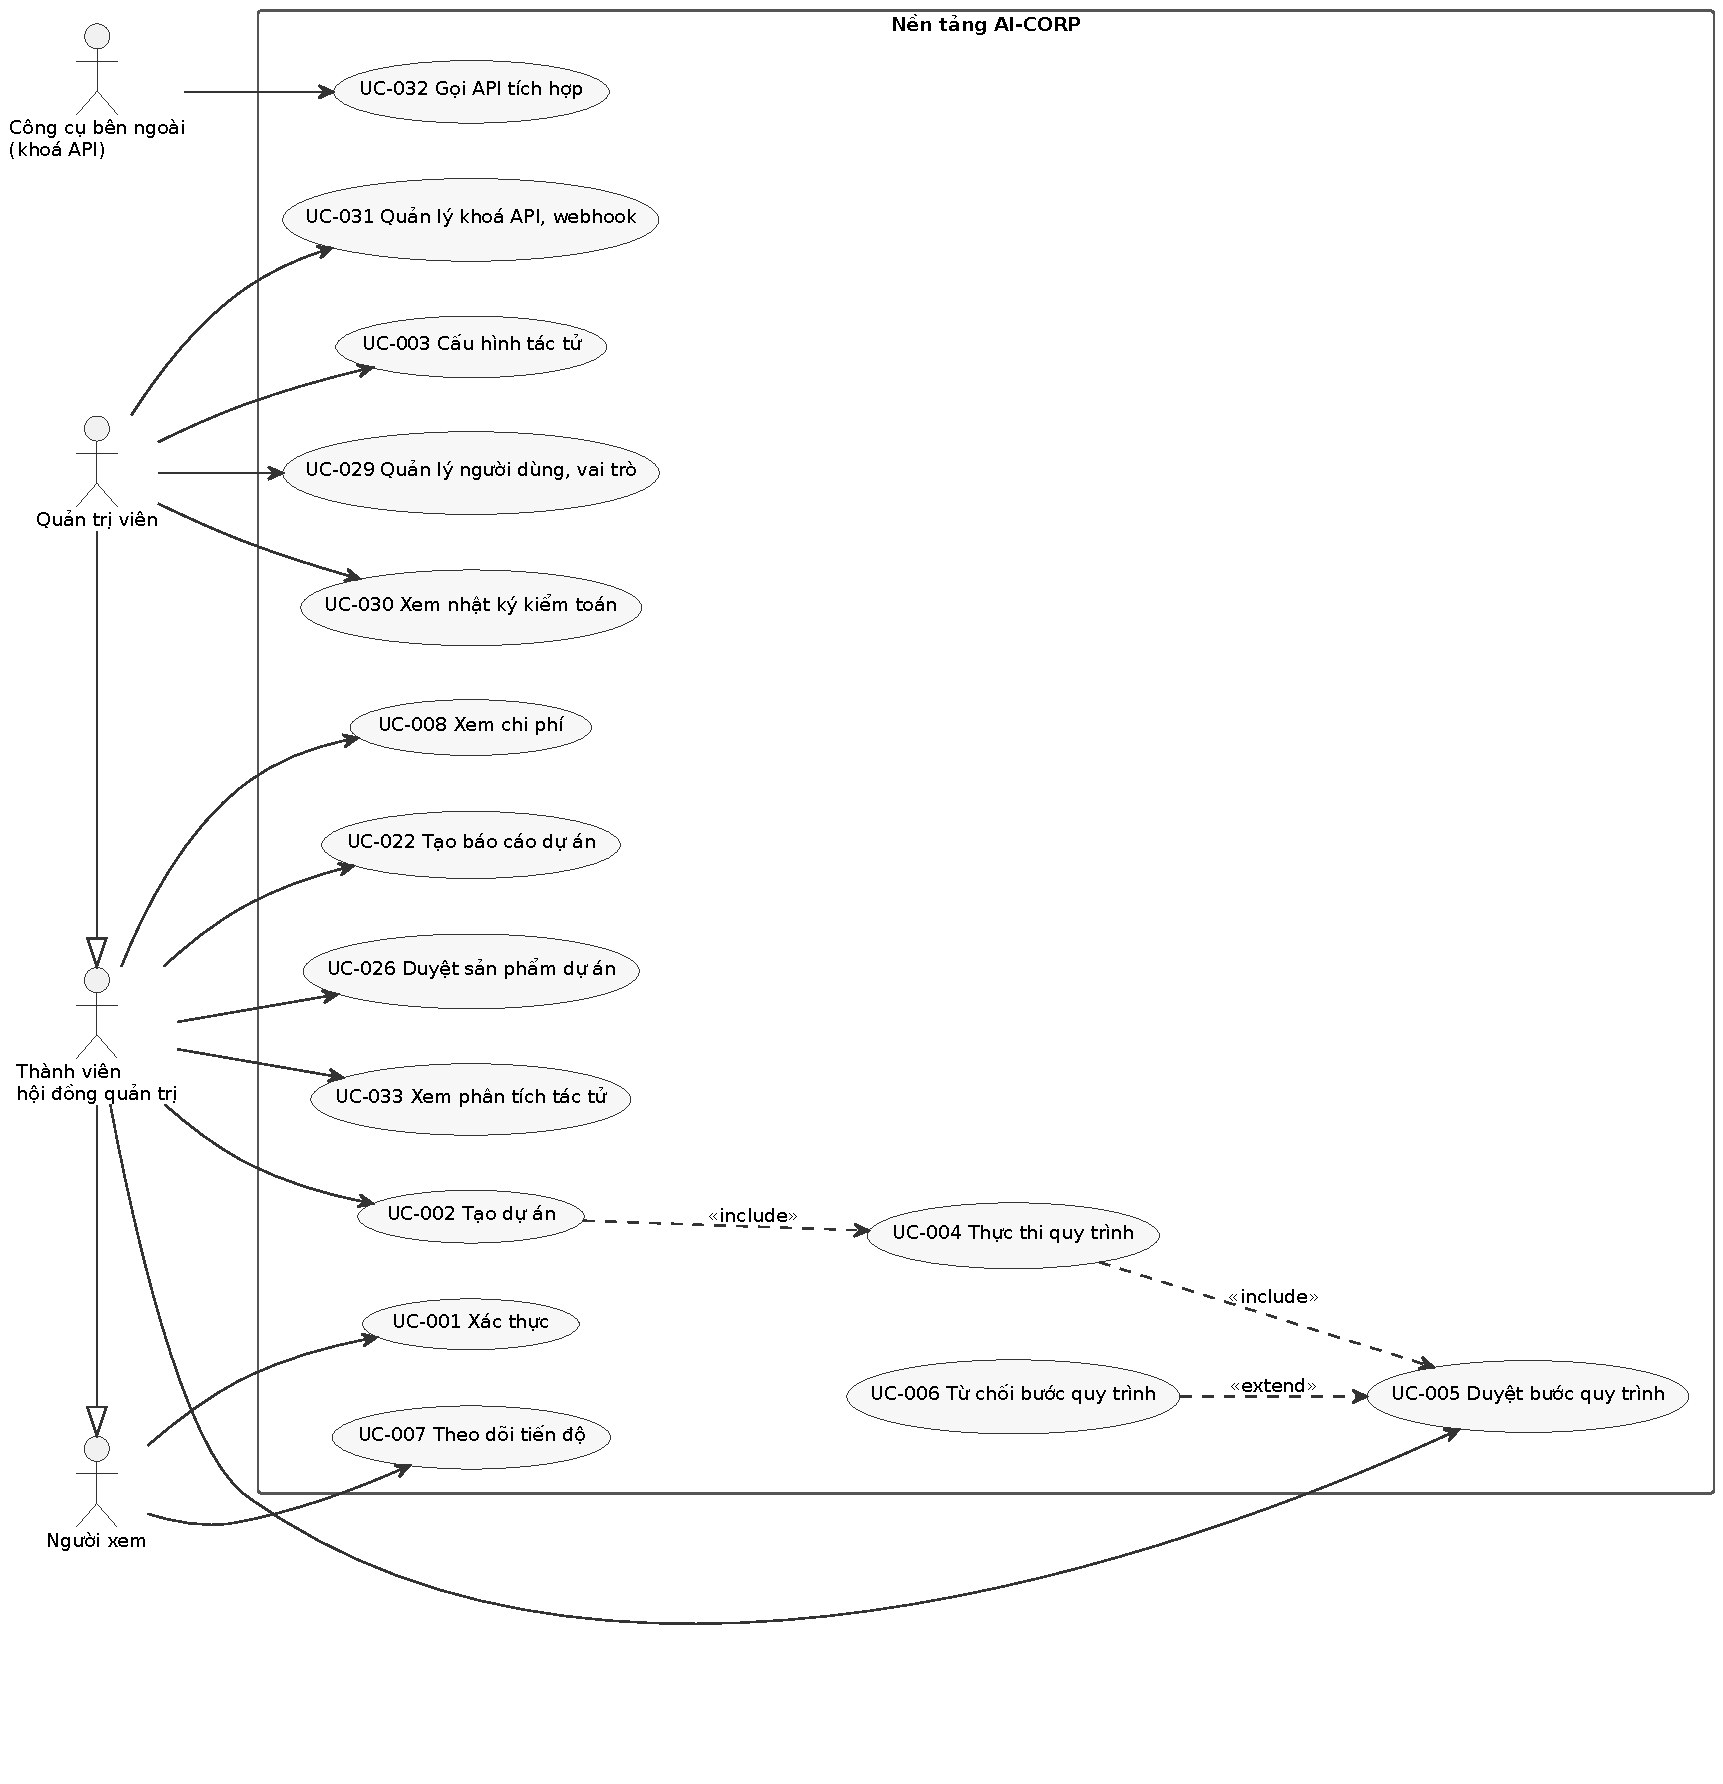
\includegraphics[width=0.92\textwidth]{sodo/use-case-con-nguoi.pdf}
\end{figure}

\begin{figure}{Sơ đồ use case phía tác tử và hệ thống}
\label{fig:uc-tac-tu}
\centering
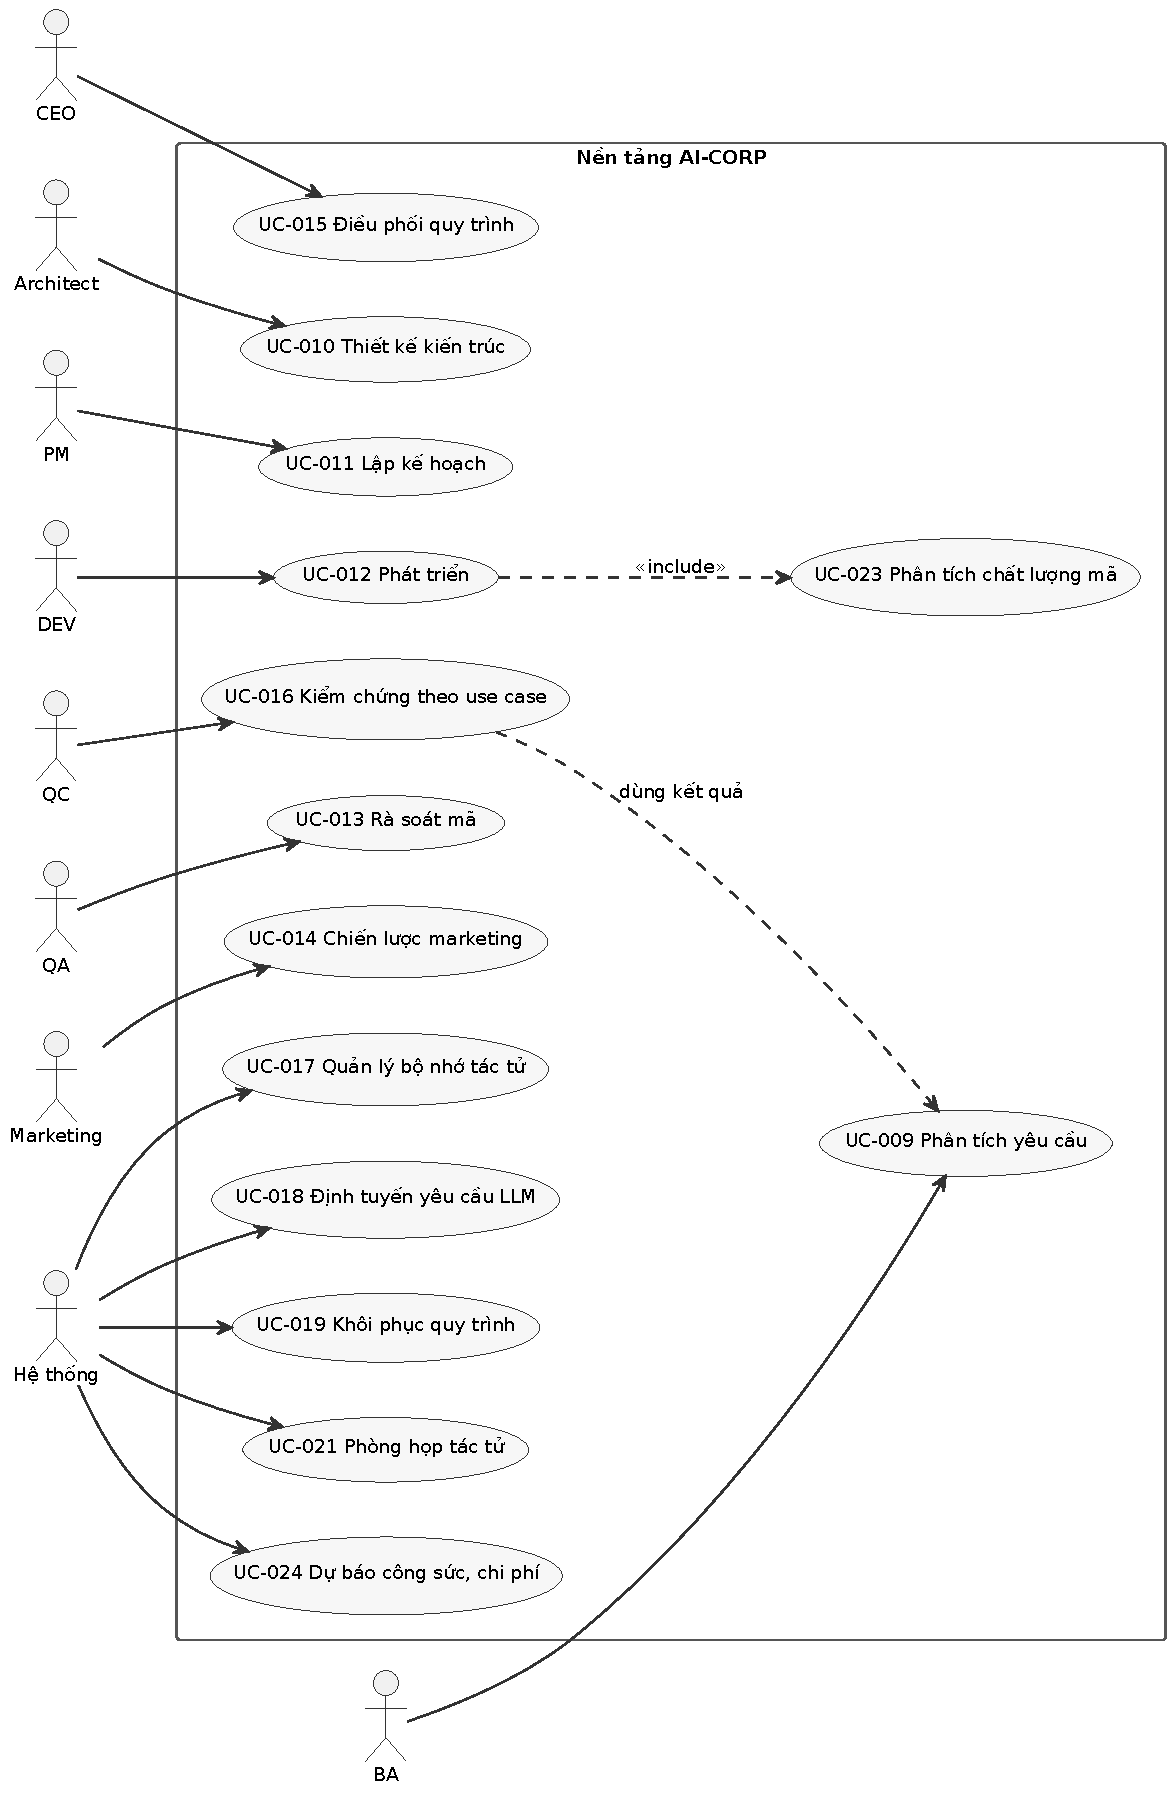
\includegraphics[width=0.68\textwidth]{sodo/use-case-tac-tu.pdf}
\end{figure}

Nhìn quan hệ giữa các use case sẽ thấy quy trình được dựng ra sao. UC-002 \textit{Tạo dự án} bao hàm UC-004 \textit{Thực thi quy trình}, vì tạo xong dự án thì quy trình chạy ngay. UC-004 bao hàm UC-005 \textit{Duyệt bước} khi quy trình có nút chờ con người, còn UC-006 \textit{Từ chối} mở rộng UC-005. UC-012 \textit{Phát triển} bao hàm UC-023 \textit{Phân tích chất lượng mã}, nơi hệ thống dự đoán phán quyết của QA và cho DEV sửa một vòng. UC-016 của QC lấy đầu ra của UC-009, tức các use case do BA viết, làm đầu vào.

\section{Đặc tả một số use case tiêu biểu}

Dưới đây là đặc tả của bốn use case đụng tới nhiều thành phần nhất. Các use case còn lại được viết theo cùng khuôn trong tài liệu yêu cầu.

\begin{table}{Đặc tả use case UC-002 Tạo dự án}
\label{tab:uc002}
\small
\begin{tabularx}{\textwidth}{|P{2.8cm}|L|}
\hline
\textbf{Tác nhân} & Thành viên hội đồng quản trị \\ \hline
\textbf{Tiền điều kiện} & Đã đăng nhập, có quyền \code{project:create} \\ \hline
\textbf{Luồng chính} &
(1) Người dùng chọn mẫu quy trình và điền tham số, ví dụ số use case tối thiểu, có bật bước phê duyệt hay không.
(2) Hệ thống kiểm tra mẫu và tham số trước khi tạo bất cứ thứ gì.
(3) Thực thể \code{Project} được tạo qua phương thức nhà máy \code{Project.create}, nơi các bất biến được áp: tên không rỗng, ngân sách dương.
(4) Dự án được lưu, sự kiện \code{ProjectCreatedEvent} được phát.
(5) Bộ máy quy trình tạo một lượt chạy gắn với phiên bản bất biến \code{mẫu@phiên_bản+băm} của định nghĩa quy trình.
(6) Hệ thống lưu một bản dự báo thời gian và chi phí lúc quy trình bắt đầu. \\ \hline
\textbf{Luồng thay thế} & Mẫu không tồn tại: trả 404. Tham số sai kiểu: trả 400 và chưa tạo dự án. Người xem gọi chức năng: trả 403 và ghi mục \code{access.denied} vào nhật ký kiểm toán. \\ \hline
\textbf{Hậu điều kiện} & Dự án ở trạng thái \code{active}, có một lượt chạy quy trình. Nhật ký kiểm toán có \code{project.create} và \code{workflow.started} \\ \hline
\end{tabularx}
\end{table}

\begin{table}{Đặc tả use case UC-004 Thực thi quy trình}
\label{tab:uc004}
\small
\begin{tabularx}{\textwidth}{|P{2.8cm}|L|}
\hline
\textbf{Tác nhân} & Hệ thống (bộ máy quy trình) và các tác tử \\ \hline
\textbf{Tiền điều kiện} & Dự án đang \code{active}, lượt chạy có định nghĩa quy trình hợp lệ \\ \hline
\textbf{Luồng chính} &
(1) Bộ máy kiểm tra ngân sách còn hay hết.
(2) Bộ máy lấy nút hiện tại và chọn chiến lược thực thi theo loại nút: \code{agent_task}, \code{sub_workflow}, \code{quality_gate}, \code{condition}, \code{parallel} hoặc \code{human_approval}.
(3) Chiến lược thực thi nút. Với nút tác tử, tác tử tương ứng chạy chu trình suy nghĩ và hành động.
(4) Bộ máy ghi một \code{WorkflowStep} kèm thời lượng, gộp kết quả vào ngữ cảnh lượt chạy và chụp ảnh trạng thái.
(5) Bộ máy chọn cạnh kế tiếp rồi lặp lại từ bước 1 cho tới khi gặp nút kết thúc. \\ \hline
\textbf{Luồng thay thế} & Nút lỗi được thử lại tối đa ba lần với thời gian chờ tăng theo hàm mũ. Vẫn lỗi thì đi theo cạnh \code{onFail}, nếu không có cạnh này thì lượt chạy chuyển \code{failed} và phát \code{workflow.failed}. Gặp nút phê duyệt: lượt chạy chuyển \code{paused}. Hết ngân sách: lượt chạy bị tạm dừng trước khi nút kế tiếp bắt đầu. \\ \hline
\textbf{Hậu điều kiện} & Lượt chạy ở \code{completed}, \code{paused}, \code{failed} hoặc \code{cancelled}. Mọi bước đã chạy đều có bản ghi và ảnh chụp \\ \hline
\end{tabularx}
\end{table}

\begin{table}{Đặc tả use case UC-005 Duyệt bước quy trình}
\label{tab:uc005}
\small
\begin{tabularx}{\textwidth}{|P{2.8cm}|L|}
\hline
\textbf{Tác nhân} & Thành viên hội đồng quản trị được giao phê duyệt \\ \hline
\textbf{Tiền điều kiện} & Lượt chạy đang dừng ở nút \code{human_approval} và có bản ghi \code{Approval} ở trạng thái \code{pending} \\ \hline
\textbf{Luồng chính} &
(1) Người dùng nhận thông báo, mở hộp thoại phê duyệt có tóm tắt sản phẩm.
(2) Người dùng bấm \textit{Approve}, giao diện gọi \code{POST /api/approvals/:id/approve}.
(3) Hệ thống kiểm tra quyền và kiểm tra người gọi đúng là người được giao.
(4) Hệ thống cập nhật phê duyệt với điều kiện trạng thái còn \code{pending}.
(5) Quyết định được ghi vào biến của lượt chạy và lượt chạy tiếp tục. \\ \hline
\textbf{Luồng thay thế} & Phê duyệt đã được trả lời trước đó: trả 409. Người không được giao hoặc người xem: trả 403, ghi \code{access.denied}. Từ chối (UC-006): bắt buộc nhập lý do, lý do được chuyển cho các tác tử chạy sau. \\ \hline
\textbf{Hậu điều kiện} & Phê duyệt có trạng thái cuối, nhật ký kiểm toán có \code{approval.approve} hoặc \code{approval.reject} \\ \hline
\end{tabularx}
\end{table}

\begin{table}{Đặc tả use case UC-016 Kiểm chứng hiện thực theo use case}
\label{tab:uc016}
\small
\begin{tabularx}{\textwidth}{|P{2.8cm}|L|}
\hline
\textbf{Tác nhân} & Tác tử QC \\ \hline
\textbf{Tiền điều kiện} & BA đã viết use case, DEV đã ghi mã vào kho tệp của dự án \\ \hline
\textbf{Luồng chính} &
(1) QC đọc use case của BA và mã của DEV.
(2) QC viết một tệp kiểm thử Jest cho mỗi use case, đặt tên \code{tests/UC-xxx.spec.ts}.
(3) Hệ thống chạy kiểm thử trong sandbox Docker, hoặc trong một bản sao tạm khi được phép chạy cục bộ.
(4) QC lập ma trận truy vết từ use case sang lớp, tệp hiện thực, tệp kiểm thử và kết quả.
(5) Độ bao phủ use case được ghi vào siêu dữ liệu OOAD của dự án. \\ \hline
\textbf{Hậu điều kiện} & Độ bao phủ chỉ tính kiểm thử đã chạy và đạt. Kiểm thử mới viết mà chưa chạy qua thì không tính. Use case chưa có kiểm thử được liệt kê là còn thiếu. \\ \hline
\end{tabularx}
\end{table}

Ở UC-005, bước (4) nhìn thì hiển nhiên nhưng lại là chỗ dễ sai nhất. Nếu hệ thống đọc trạng thái, thấy \code{pending}, rồi mới ghi, thì hai yêu cầu đến gần như cùng lúc sẽ cùng thấy \code{pending} và cùng ghi thành công. Lỗi này đã xảy ra thật, và chương~\ref{chap:kiem-thu} kể lại nó được sửa thế nào.

\section{Mô hình miền}

Mô hình miền của nền tảng xoay quanh ba aggregate chính, thể hiện ở Hình~\ref{fig:mo-hinh-mien}:

\begin{itemize}
\item \textbf{Project} là gốc aggregate, chứa các \code{Milestone} và \code{Task}. Ngân sách và chi phí đã tiêu được biểu diễn bằng value object \code{Money}. Trạng thái \code{ProjectStatus} cũng là một value object có quy tắc chuyển trạng thái riêng.
\item \textbf{Agent} có vai trò \code{AgentRole}, cấu hình mô hình LLM, bộ nhớ \code{AgentMemory} và máy trạng thái vòng đời.
\item \textbf{WorkflowRun} tham chiếu tới một phiên bản bất biến của định nghĩa quy trình, chứa các \code{WorkflowStep} và ảnh chụp \code{WorkflowSnapshot}, có thể có lượt chạy cha (khi là quy trình con) và các \code{Approval}.
\end{itemize}

Xung quanh còn có các khái niệm phụ trợ. Có \code{User} và \code{Role}, có \code{AuditLog} chỉ cho ghi thêm chứ không cho sửa. Có \code{ApiKey}, \code{Webhook} và \code{WebhookDelivery}, có \code{ApiUsageLog} lưu chi phí từng lời gọi LLM, rồi \code{QualityGateLog} và \code{ProjectEstimate}. Cuối cùng là aggregate \code{LlmProviderConfig} quản lý danh sách \code{LlmModel} của nó.

\begin{figure}{Mô hình miền rút gọn của nền tảng}
\label{fig:mo-hinh-mien}
\centering
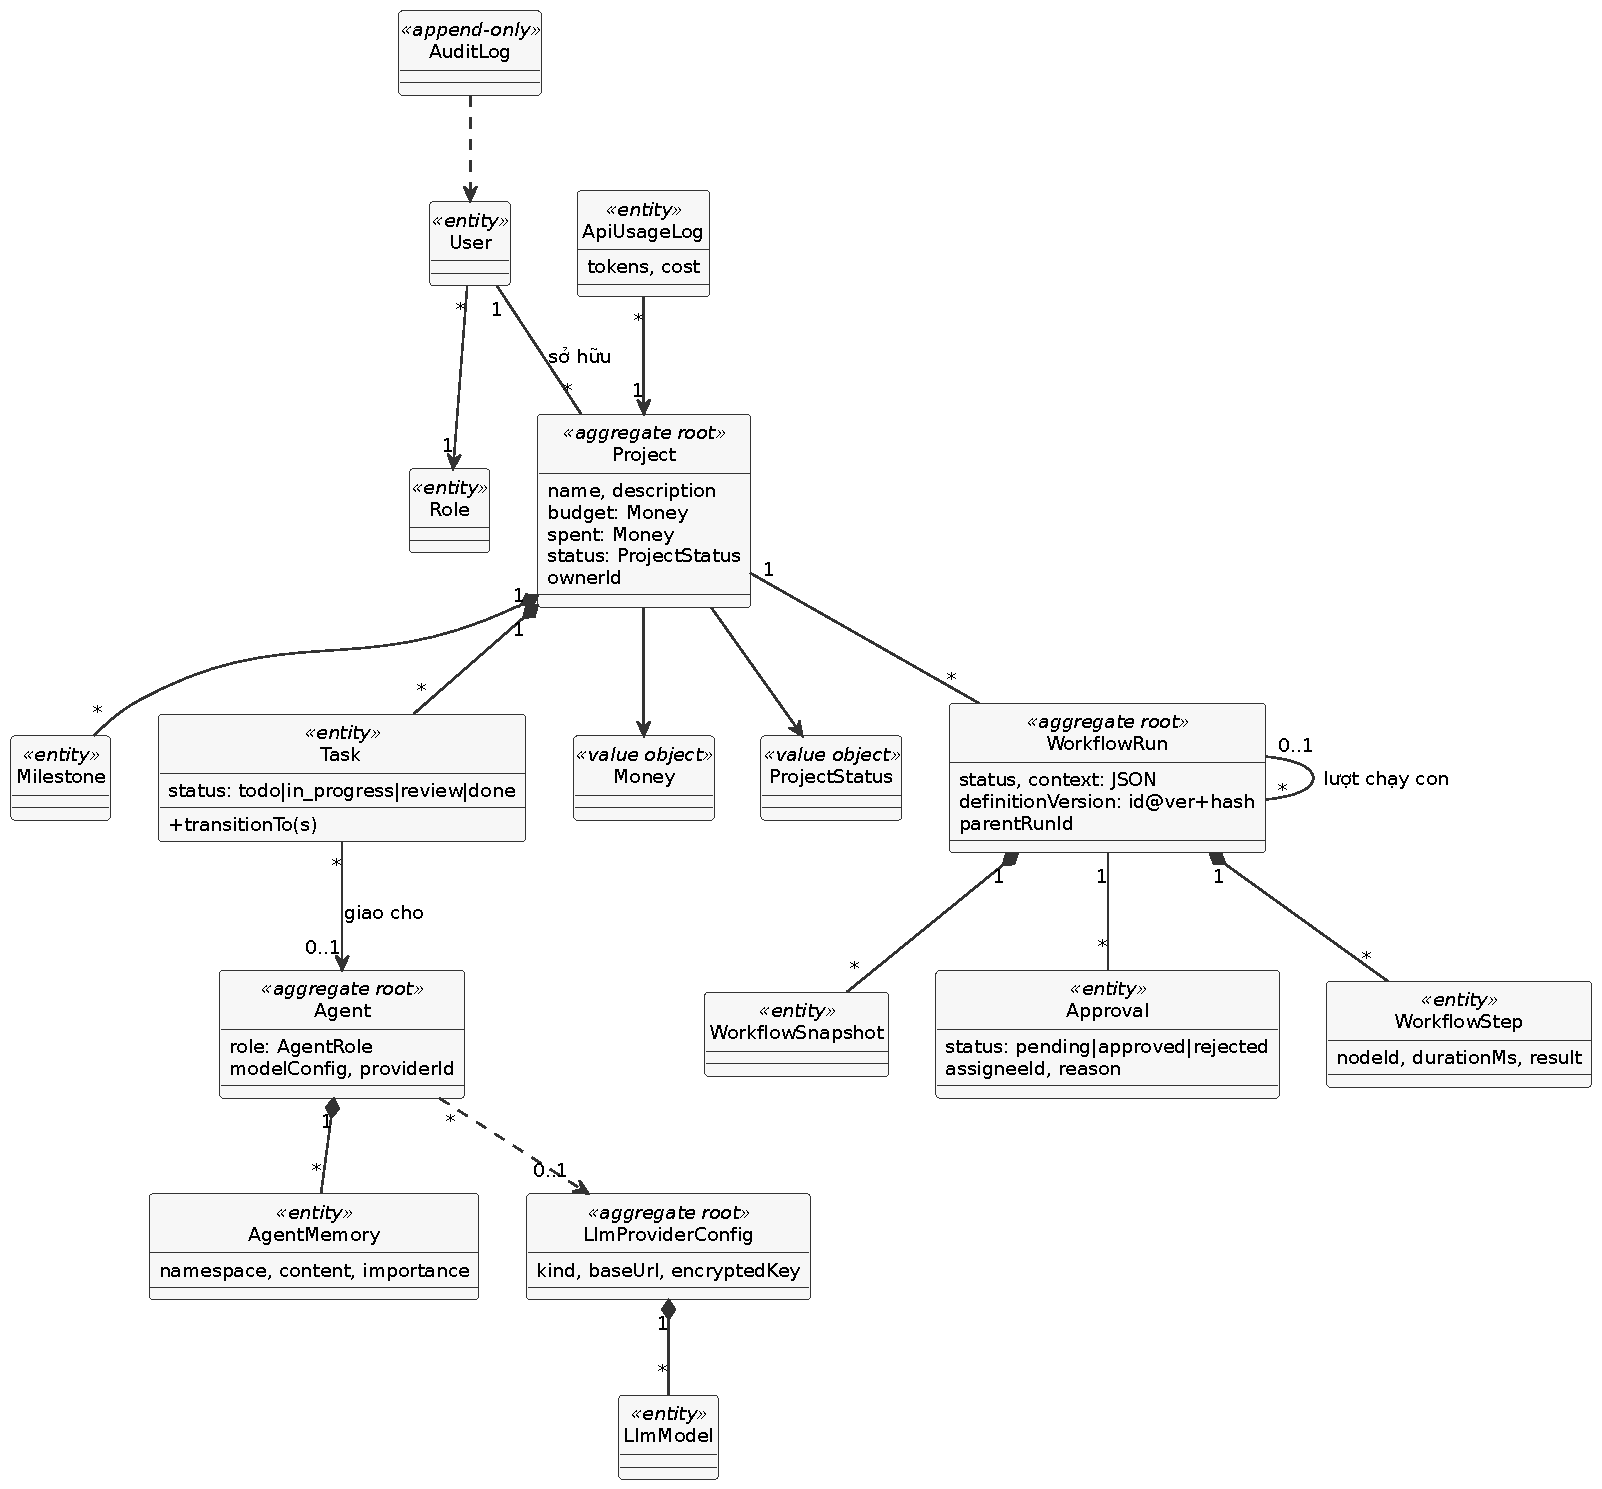
\includegraphics[width=\textwidth]{sodo/mo-hinh-mien.pdf}
\end{figure}
